\documentclass[10pt]{beamer}
\usetheme{PaloAlto}
\usecolortheme{seahorse}
\setbeamertemplate{navigation symbols}{}
\setbeamertemplate{enumerate items}[square]
\setlength{\parskip}{\baselineskip}


\usepackage[english]{babel}
\usepackage[utf8]{inputenc}
\usepackage[T1]{fontenc}
\usepackage{microtype}
\usepackage{todonotes}
\usepackage{graphicx}
\usepackage{times}

\usepackage[english]{isodate}
\isodate


\title{Comparing Deep Learning Models for Lightning Strike Prediction in a Changing Climate}
\subtitle{An Empirical Study}
\author{NAME REDACTED}
\institute{Blekinge Institute of Technology}
\date{\today}


\begin{document}


\begin{frame}
\titlepage
\end{frame}

\begin{frame}{Outline}
\tableofcontents
\end{frame}


\section{Purpose and Objectives}


\begin{frame}{Purpose and objectives}
\centering
\begin{description}
	\item[Academic] Evaluate and compare the performance of multiple deep learning models for lightning strike prediction across different timeframes.
	\item[Practical] Construction of a practically applicable model for lightning strike prediction.
\end{description}
\end{frame}


\begin{frame}{Importance}
Many practical applications:
\begin{itemize}
	\item \textbf{Early warning systems:} Evacuations can be initiated sooner, airline travel will be safer, etc.
	\item \textbf{Efficient resource allocation:} Standby personal, planning vehicle routes, etc.
	\item \textbf{Assess environmental impact:} Detection of lightning-induced wildfires, stormwater runoff, soil erosion.
\end{itemize}
\end{frame}


\begin{frame}{The Problem}
Current methods largely relies on numerical models and simulations.
\begin{itemize}
	\item Requires a large and complex network of sensors.
	\item Requires massive computational resources on a centralized system.
	\item Requires cooperation on a global scale, meaning large communication overhead.
\end{itemize}
Deep learning might be a better way.
\end{frame}


\begin{frame}{Research Questions}
Too achieve the objectives, the following research questions were proposed:
\begin{enumerate}
	\item \textit{\textbf{How does the proposed models perform across different time frames?}}
	\item \textit{Which of the proposed models are most effective for predicting lightning strikes, and how do they compare to each other?}
	\item \textit{Which are the optimal features and input data for predicting lightning strikes?}
	\item \textit{What are the optimal hyperparameters and model configurations for predicting lightning strikes?}
	\item \textit{What are the challenges and limitations of using deep learning for lightning prediction, and how can these limitations be mitigated?}
\end{enumerate}
\end{frame}


\section{Datasets}


\begin{frame}{Data source}
All data is curated by the \textit{Swedish Meteorological and Hydrological Institute} (SMHI).\newline
Why?
\begin{itemize}
	\item As SMHI is an official governmental agency, the data is likely legitimate and unbiased.
	\item As the data is open and publicly available, it is likely free and reproducable.
	\item Low-level error handling can be outsourced, further increasing its viability.
\end{itemize}
\end{frame}


\begin{frame}{Data Overview}
In total, two datasets were utilized:
\begin{enumerate}
	\item The \textit{Lightning Archive} (LIGHT dataset), a collection of all lightning strikes occured in sweden, used as labels.
	\item The \textit{Meteorological Analysis Model data} (MESAN dataset), a collection of meteorological data, used as features.
\end{enumerate}
\end{frame}


\begin{frame}{LIGHT Overview}
The LIGHT dataset is a collection of lightning strikes that occured in Sweden since January 2, 2012.
\par
Has been subjected to initial cleaning procedures and error handling, such as
\begin{itemize}
	\item Interpolation
	\item Chi-Square filter
\end{itemize}
\vspace{0.5cm}
\begin{alertblock}{Dynamism}
	Even though the underlying data is static, the measured data is dynamic.
	Data is available from before 2012, but before this it was collected on different sensors and hardware.
\end{alertblock}
\end{frame}


%\begin{frame}{LIGHT Format}
%\begin{columns}
%	\column{0.5\textwidth}
%	\begin{itemize}
%		\item Stored in JSON files.
%		\item Each file represents a day.
%		\item Follows the \textit{Universal ASCII Lightning Format} (UALF).
%		\item Can be significantly compressed as the columns make up for a large portion of the file size.
%	\end{itemize}
%	\column{0.5\textwidth}
%	Includes parameters such as:
%	\begin{itemize}
%		\item Timestamp
%		\item Lat/lon position
%		\item Peak current
%		\item Number of Sensors
%		\item Degrees of Freedom
%		\item Ellipse Angle
%		\item Chi Square Value
%		\item ...
%	\end{itemize}
%\end{columns}
%\end{frame}


\begin{frame}{LIGHT Visualization}
\begin{figure}
	\label{light-analysis}
	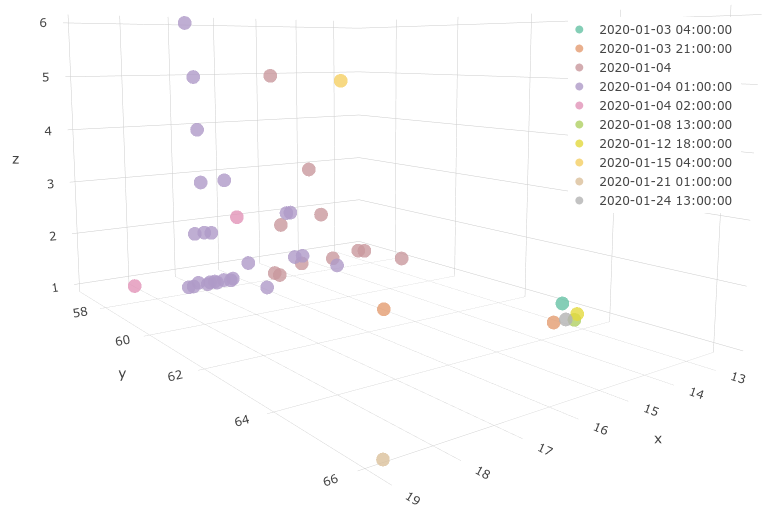
\includegraphics[width=0.9\textwidth]{figures/light-analysis}
	\caption{Visualization of the LIGHT dataset during January 2020.}
\end{figure}
\end{frame}


\begin{frame}{LIGHT Analysis}
The graph illustrates that lightning strikes tend to occur both in close temporal and spacial proximity.

Careful when analyzing labels to not include any "hints" about the testing data.
\end{frame}


\begin{frame}[shrink=13]{LIGHT Preprocessing}
\begin{enumerate}
	\item \textbf{Filtering:} The data was geographically restricted due to limited computational resources.
		\begin{itemize}
			\item Filter applied to the vicinity of Linköping $\pm 300 km$.
			\item Resulting in a total area of $90000 km^2$.
			\item Might enhance the model accuracy as the topology remains largely the same.
		\end{itemize}
	\item \textbf{Balancing:} An even ratio of positive/negative instances is preferred.
		\begin{enumerate}
			\item Negative instances were randomly generated.
			\item Discarded if they didn't adhere to previous filters.
			\item Discarded if they were already present in the positive dataset.
			\item Otherwise added to the dataset.
			\item Repeated until the positive/negative instance ratio was 50/50.
		\end{enumerate}
	\item \textbf{Binning:} The data was clustered to maximize variability.
		\begin{itemize}
			\item Useful because many positive instances are very similar.
			\item Achieved by flooring every timestamp to the nearest hour and coordinates to a specific number of decimals.
			\item Duplicate instances were deleted, favoring positive instances to maximize data size. Afterwards the classes were rebalanced.
			\item In this study 0 decimals were used, resulting in a bin size of $555.6 km$, covering the entire geographic area.
			\item A higher decimal count would likely be beneficial.
		\end{itemize}
\end{enumerate}
\end{frame}


\begin{frame}{MESAN Overview}
Contains the meteorological data used as input or features to the models.
\par
Released on hourly intervals.
\par
Encompassing $11,679,839 km^2$, including Scandinavia, the Baltic States and the Northern part of Europe.
\par
Available from December 2014. Before that, other hardware was used.
\par
Big data, exceeding a terrabyte in size.
\end{frame}


\begin{frame}[shrink=10]{MESAN Parameters}
The following parameters are included in the MESAN dataset:
\begin{columns}
	\column{0.5\textwidth}
	\begin{itemize}
		\item Pressure
		\item Temperature
		\item Wet bulb temperature
		\item Maximum temperature
		\item Minimum temperature
		\item Visibility
		\item Wind gust
		\item U-component of wind
		\item V-component of wind
		\item Relative humidity
		\item Total cloud cover
		\item Low cloud cover
		\item Medium cloud cover
		\item High cloud cover
		\item Fraction of significant clouds
	\end{itemize}
	\column{0.5\textwidth}
	\begin{itemize}
		\item Cloud base of significant clouds above ground
		\item Cloud base of significant clouds above sea
		\item Cloud Top of significant clouds
		\item Frozen part of total precipitation
		\item Type of precipitation
		\item Sort of precipitation
		\item 12 hour precipitation
		\item 24 hour precipitation
		\item 1 hour precipitation
		\item 3 hour precipitation
		\item 12 hour snow
		\item 24 hour snow
		\item 1 hour snow
		\item 3 hour snow
	\end{itemize}
\end{columns}
\end{frame}


\begin{frame}{MESAN Format}
Stored in \textit{Gridded Binary}, or GRIB files.
\par
In order to minimize the distance disparity between grid points, grids and parameters in the files released by SMHI are rotated according to a Lambert projection.
\par
However, the wind vectors can be left unrotated as the rotation remains the same for all files, and because it is their relationship to the rest of the data that matters.
\end{frame}


%\begin{frame}{GRIB Structure}
%\begin{itemize}
%	\item Each GRIB file contains a number of optional parameters, commonly called "messages".
%	\item Each message contains metadata as well as multi-dimensional arrays.
%	\item The arrays serve as a spatial grid of collected measurements.
%\end{itemize}
%\end{frame}


\begin{frame}{MESAN Exploratory analysis}
To get an overview of the data, an exploratory analysis was conducted:
\begin{itemize}
\item The dataset is missing a lot of values, with the "minimum/maximum temperate" being non-existent.
\item Compound parameters such as "24-hour precipitation" are not continuous and misses values except for on the specific intervals.
\end{itemize}
\end{frame}


\begin{frame}{MESAN Correlation analysis}
To decrease data processing and limit model confusion, the input data should be independent.
\par
A \textit{covariance matrix} was used to find similar parameters:
\begin{enumerate}
	\item A Shapiro-Wilk test with $\alpha=0.05$ was used on all parameters to check for normality.
	\item All parameters were normalized.
	\item The Spearman's rank correlation coefficient was used to build the matrix.
\end{enumerate}
\end{frame}


\begin{frame}{Covariance Matrix (pre)}
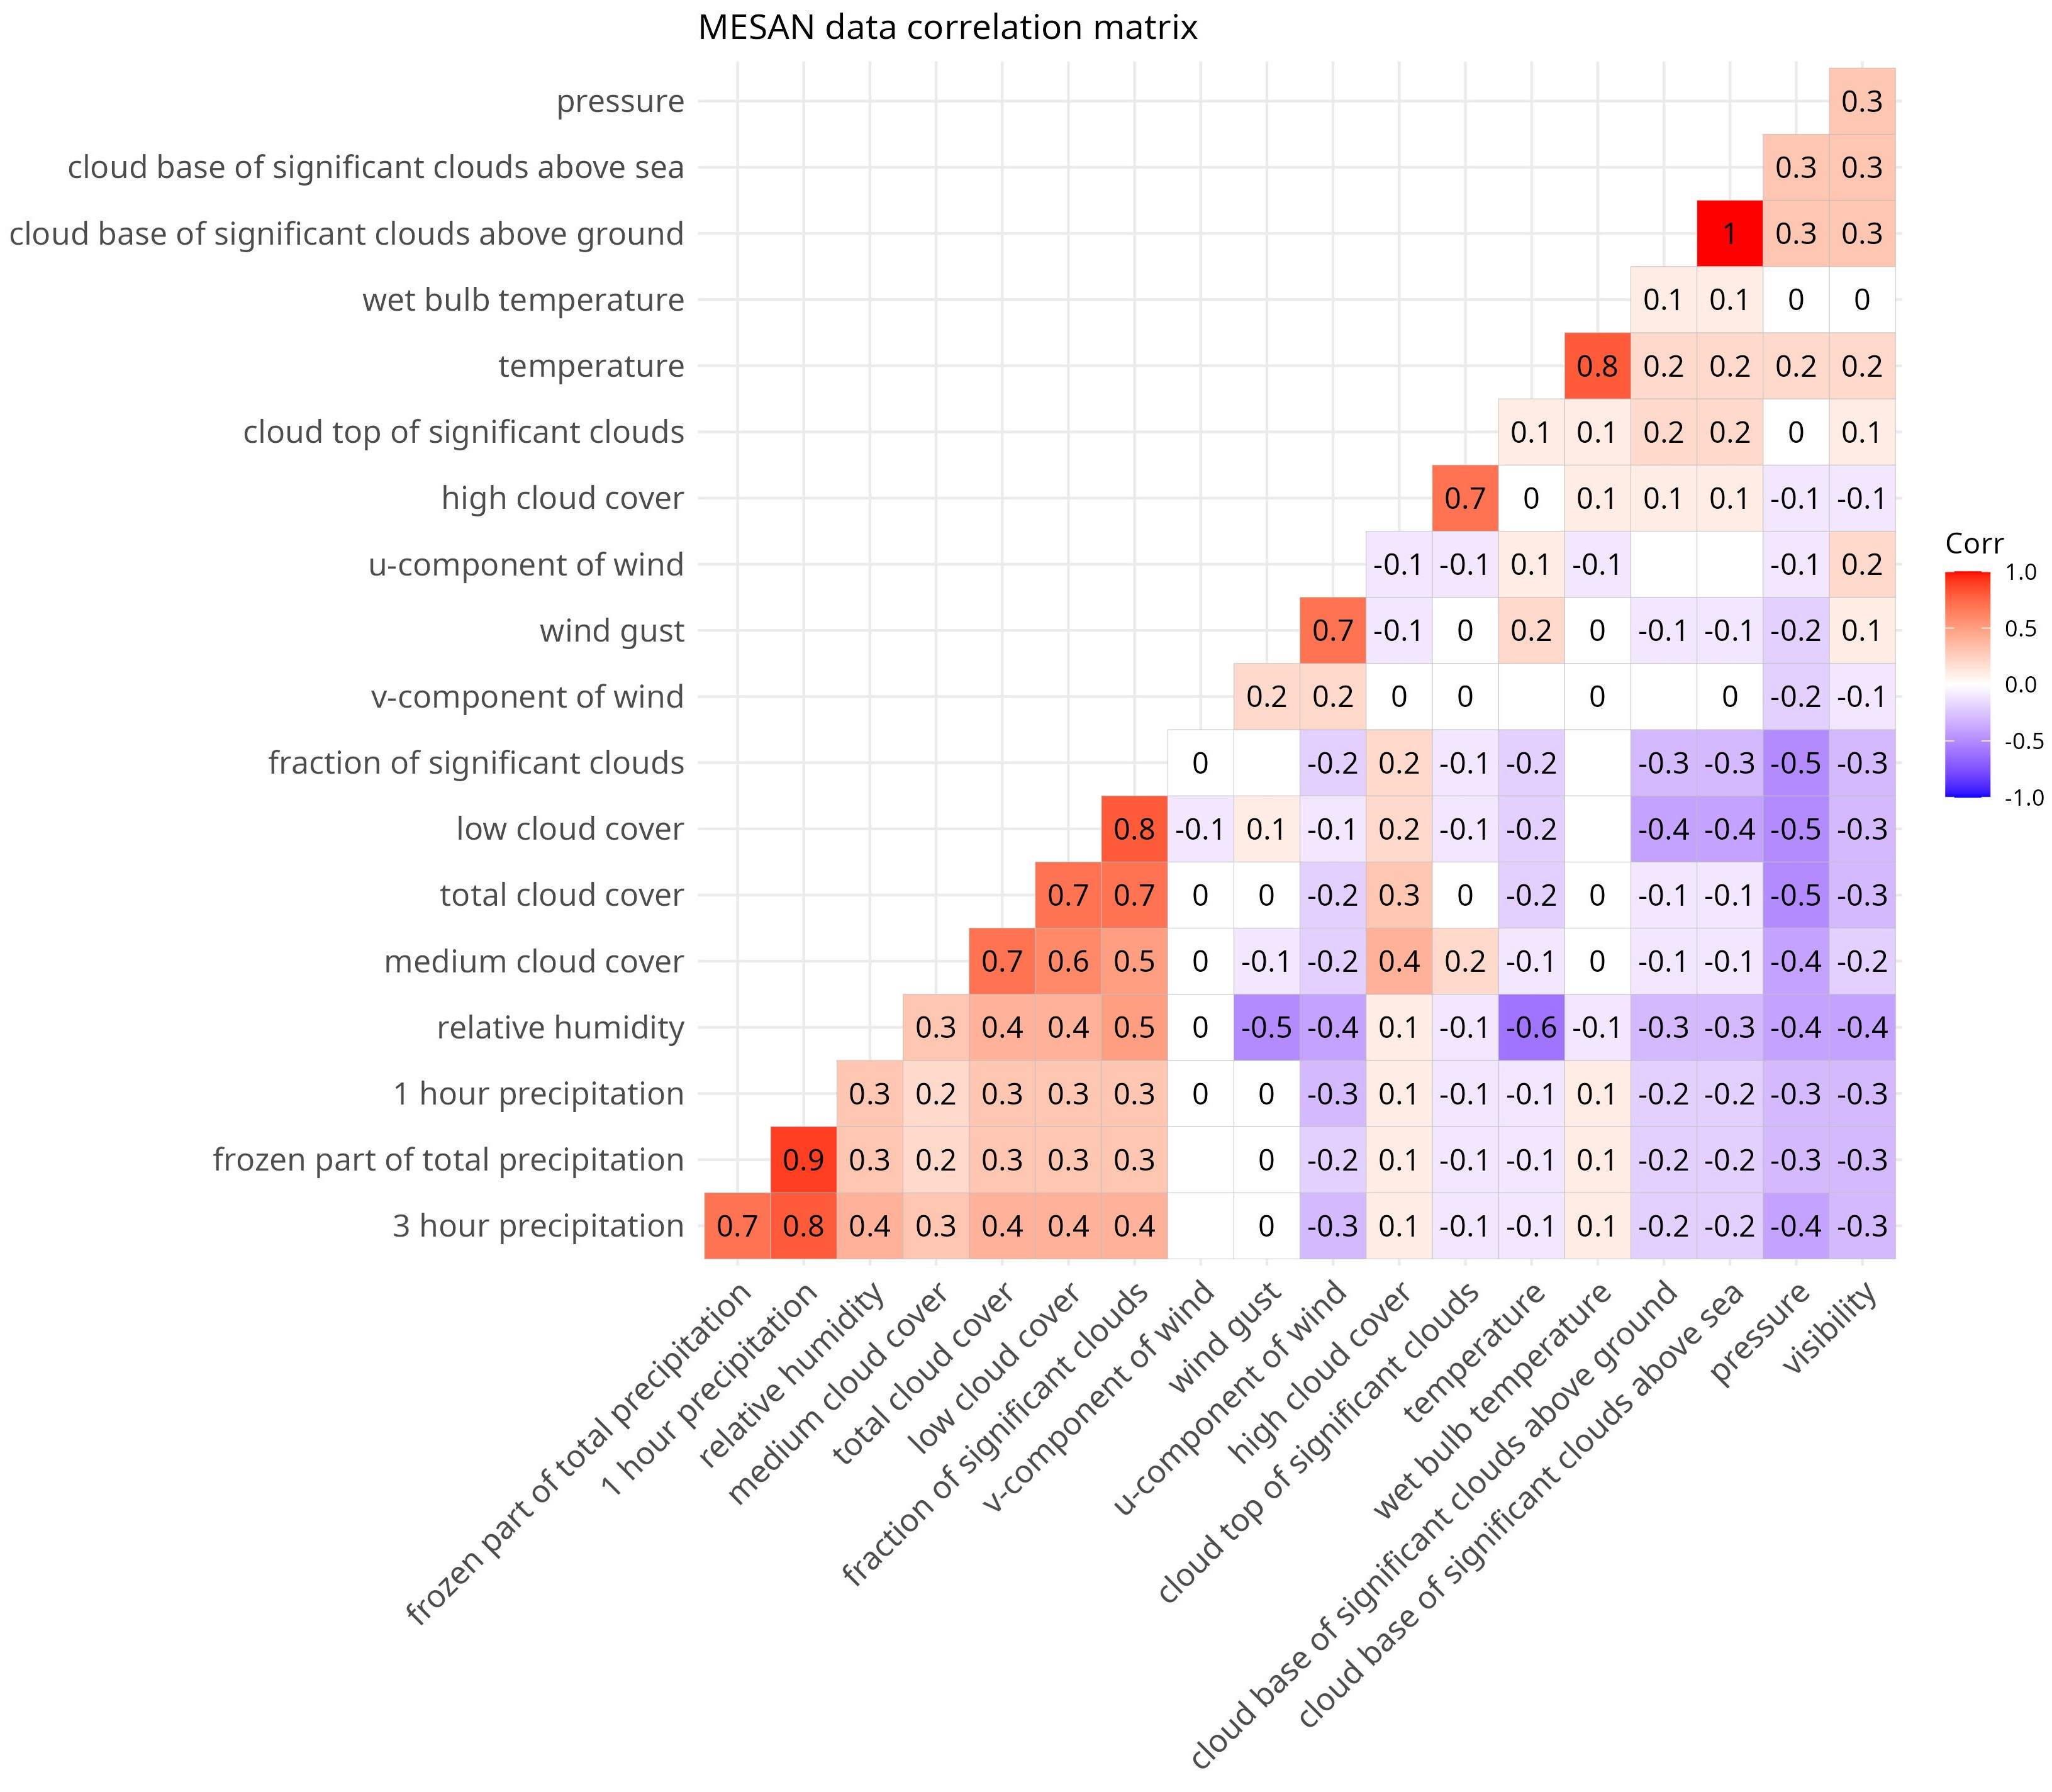
\includegraphics[width=0.85\textwidth]{figures/mesan-analysis-matrix-pre}
\end{frame}


\begin{frame}{MESAN Correlation analysis}
Based on the correlation matrix, the following parameters were removed in favor of more independent features:
\begin{itemize}
	\item Wet-bulb temperature
	\item Cloud base of significant clouds above sea
	\item Total cloud cover
	\item Wind gust
\end{itemize}
\end{frame}


\begin{frame}{Covariance Matrix (post)}
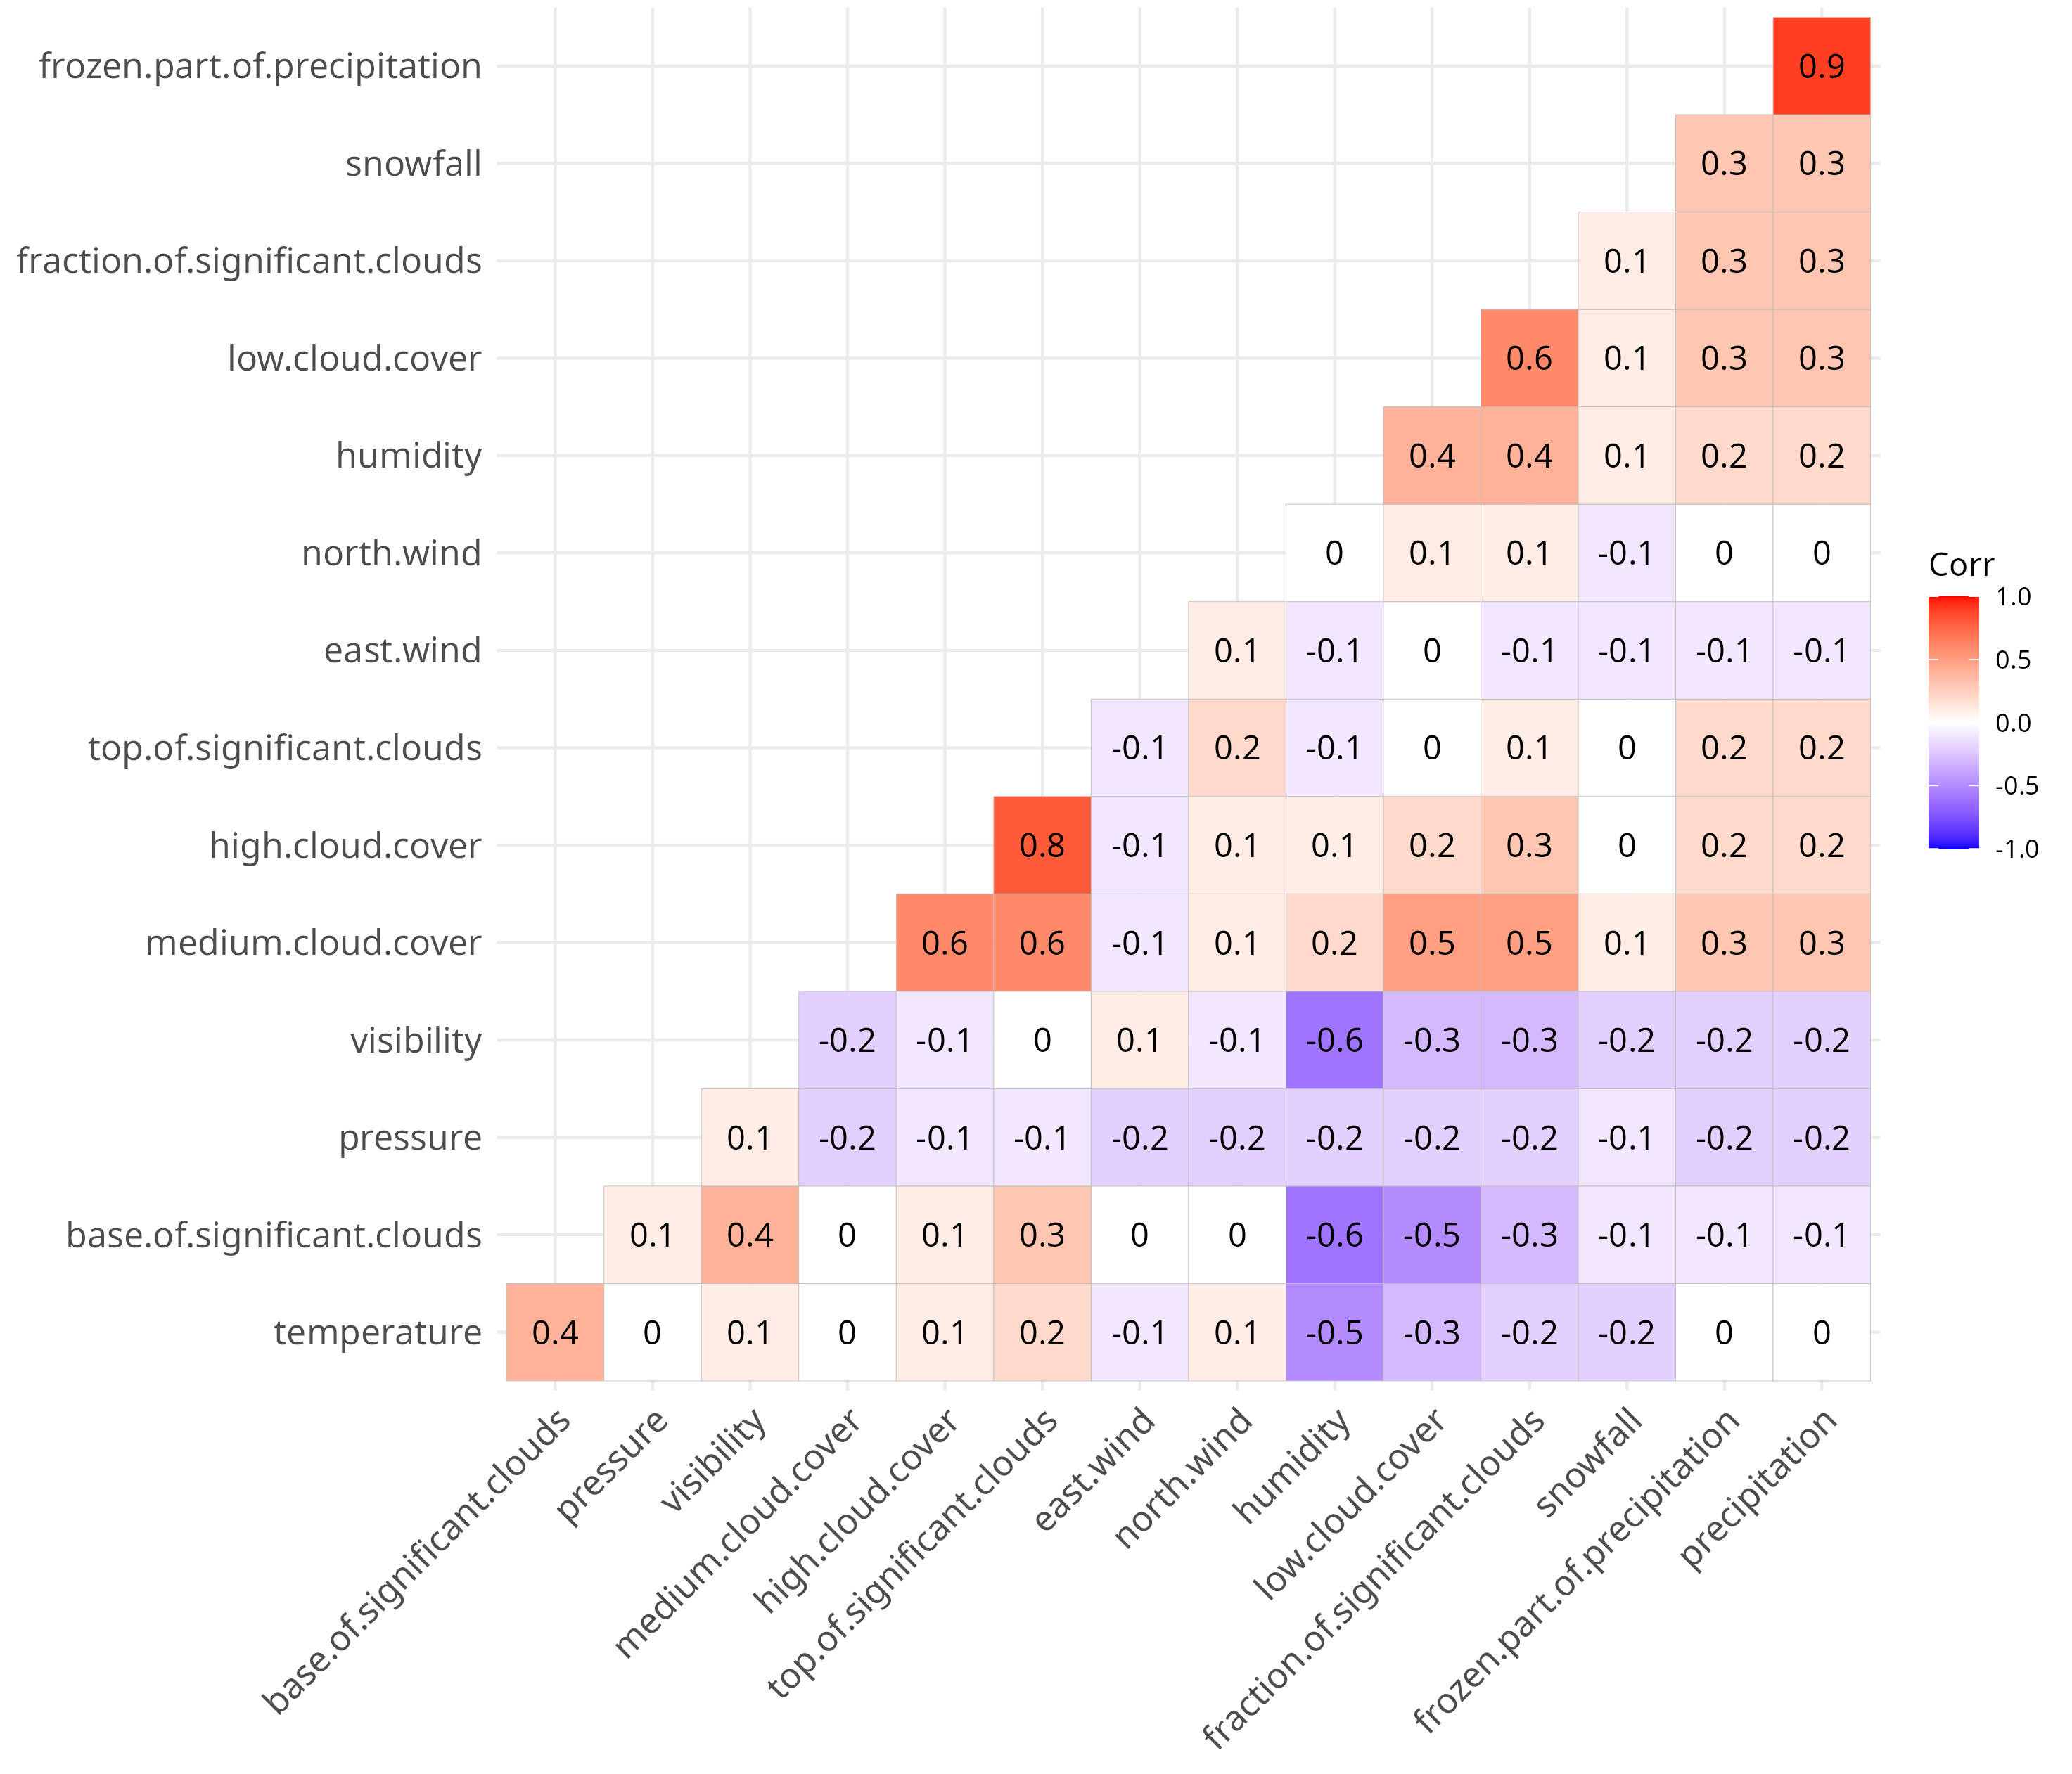
\includegraphics[width=0.9\textwidth]{figures/mesan-analysis-matrix-post}
\end{frame}


\begin{frame}{MESAN PC Analysis}
A \textit{Principal Component Analysis}, or PCM, was used to determine the parameters with highest importance.
\par
It can be used to minimize the number of input parameters while retaining the maximum information amount.
\par
The PCA process yields a set of vectors, ranked in order of their impact on the overall variance of the dataset.
\end{frame}


\begin{frame}{MESAN PCA Table}
\begin{table}[h]
	\centering
	\begin{tabular}{c|c|c|c}
		\textbf{Parameter} & \textbf{PC1} & \textbf{PC2} & \textbf{PC3} \\
		\hline \hline
		pressure                       & -0.21 & -0.02 & -0.02 \\
		\hline
		temperature                    & -0.15 &  0.37 & -0.10 \\
		\hline
		visibility                     & -0.28 &  0.15 &  0.08 \\
		\hline
		east.wind                      & -0.04 & -0.08 &  0.18 \\
		\hline
		north.wind                     &  0.09 &  0.12 &  0.17 \\
		\hline
		humidity                       &  0.32 & -0.28 &  0.07 \\
		\hline
		low.cloud.cover                &  0.39 & -0.15 &  0.21 \\
		\hline
		medium.cloud.cover             &  0.37 &  0.25 &  0.22 \\
		\hline
		high.cloud.cover               &  0.28 &  0.43 &  0.17 \\
		\hline
		fraction.of.significant.clouds &  0.37 & -0.06 &  0.20 \\
		\hline
		base.of.significant.clouds     & -0.21 &  0.43 & -0.05 \\
		\hline
		top.of.significant.clouds      &  0.17 &  0.51 &  0.11 \\
		\hline
		frozen.part.of.precipitation   &  0.30 &  0.08 & -0.55 \\
		\hline
		precipitation                  &  0.25 &  0.09 & -0.56 \\
		\hline
		snowfall                       &  0.13 & -0.04 & -0.35 \\
	\end{tabular}
	\label{tbl:pcx}
\end{table}
\end{frame}


\begin{frame}{MESAN PCA Results}
\begin{itemize}
	\item The data is relatively independent as 12/15 PCs are required for 95\% comprehensiveness.
	\item PC1 is dispersely influenced, but primarily by cloud related parameters ("low/medium cloud cover" and "fraction of significant clouds").
	\item PC2 is similarly comprised of cloud related parameters ("base/top of significant clouds" and "high cloud cover").
	\item PC3 is influenced by precipitation related parameters ("precipitation" and "frozen part of precipitation").
	\item The least important parameters seem to include "snowfall", "temperature" and wind-related parameters.
\end{itemize}
\end{frame}


\begin{frame}{MESAN Preprocessing}
\begin{enumerate}
\item \textbf{Extraction:} The data had to be extracted from the GRIB files.
	\begin{enumerate}
		\item For each lightning strike a trailing sequence of 73 weather observations were extracted.
		\item The coordinates for each lightning strike was rotated.
		\item A mean of all metrics gathered within a 3 km radius were calculated.
		\item If no metrics were found, the radius was incrementally expanded up to 6 km.
		\item If no value was found, it was labelled as missing.
	\end{enumerate}
\item \textbf{Imputation:} After extraction the dataset contained multiple missing values.
	\begin{itemize}
		\item Missing values were derived from the closest known value, either forwards or backwards in time.
		\item Group boundaries were kept to ensure no imputation from other lightning strikes occured.
	\end{itemize}
\end{enumerate}
\end{frame}


\section{Model Selection}


\begin{frame}{DNNs}

\textit{Dense Neural Networks}, or DNNs, are the most basic type of DL model.
\begin{itemize}
	\item Has an input layer, an output layer, and at least one hidden layer in between.
	\item The input layer varies depending on the input parameters.
	\item The output layer varies depending on the purpose and goal of the model.
\end{itemize}
\vspace{0.5cm}
\begin{columns}
	\column{0.5\textwidth}
	\begin{center} 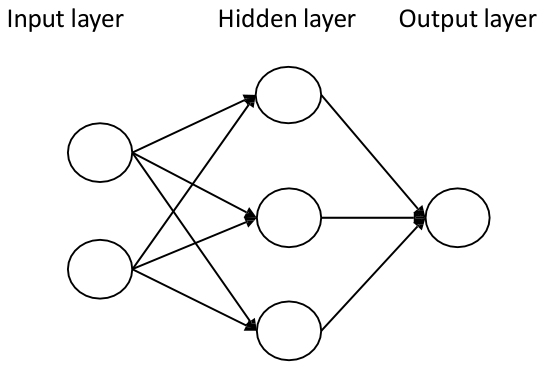
\includegraphics[width=0.8\textwidth]{figures/dnn-simple} \end{center}
	\column{0.5\textwidth}
	\begin{center} 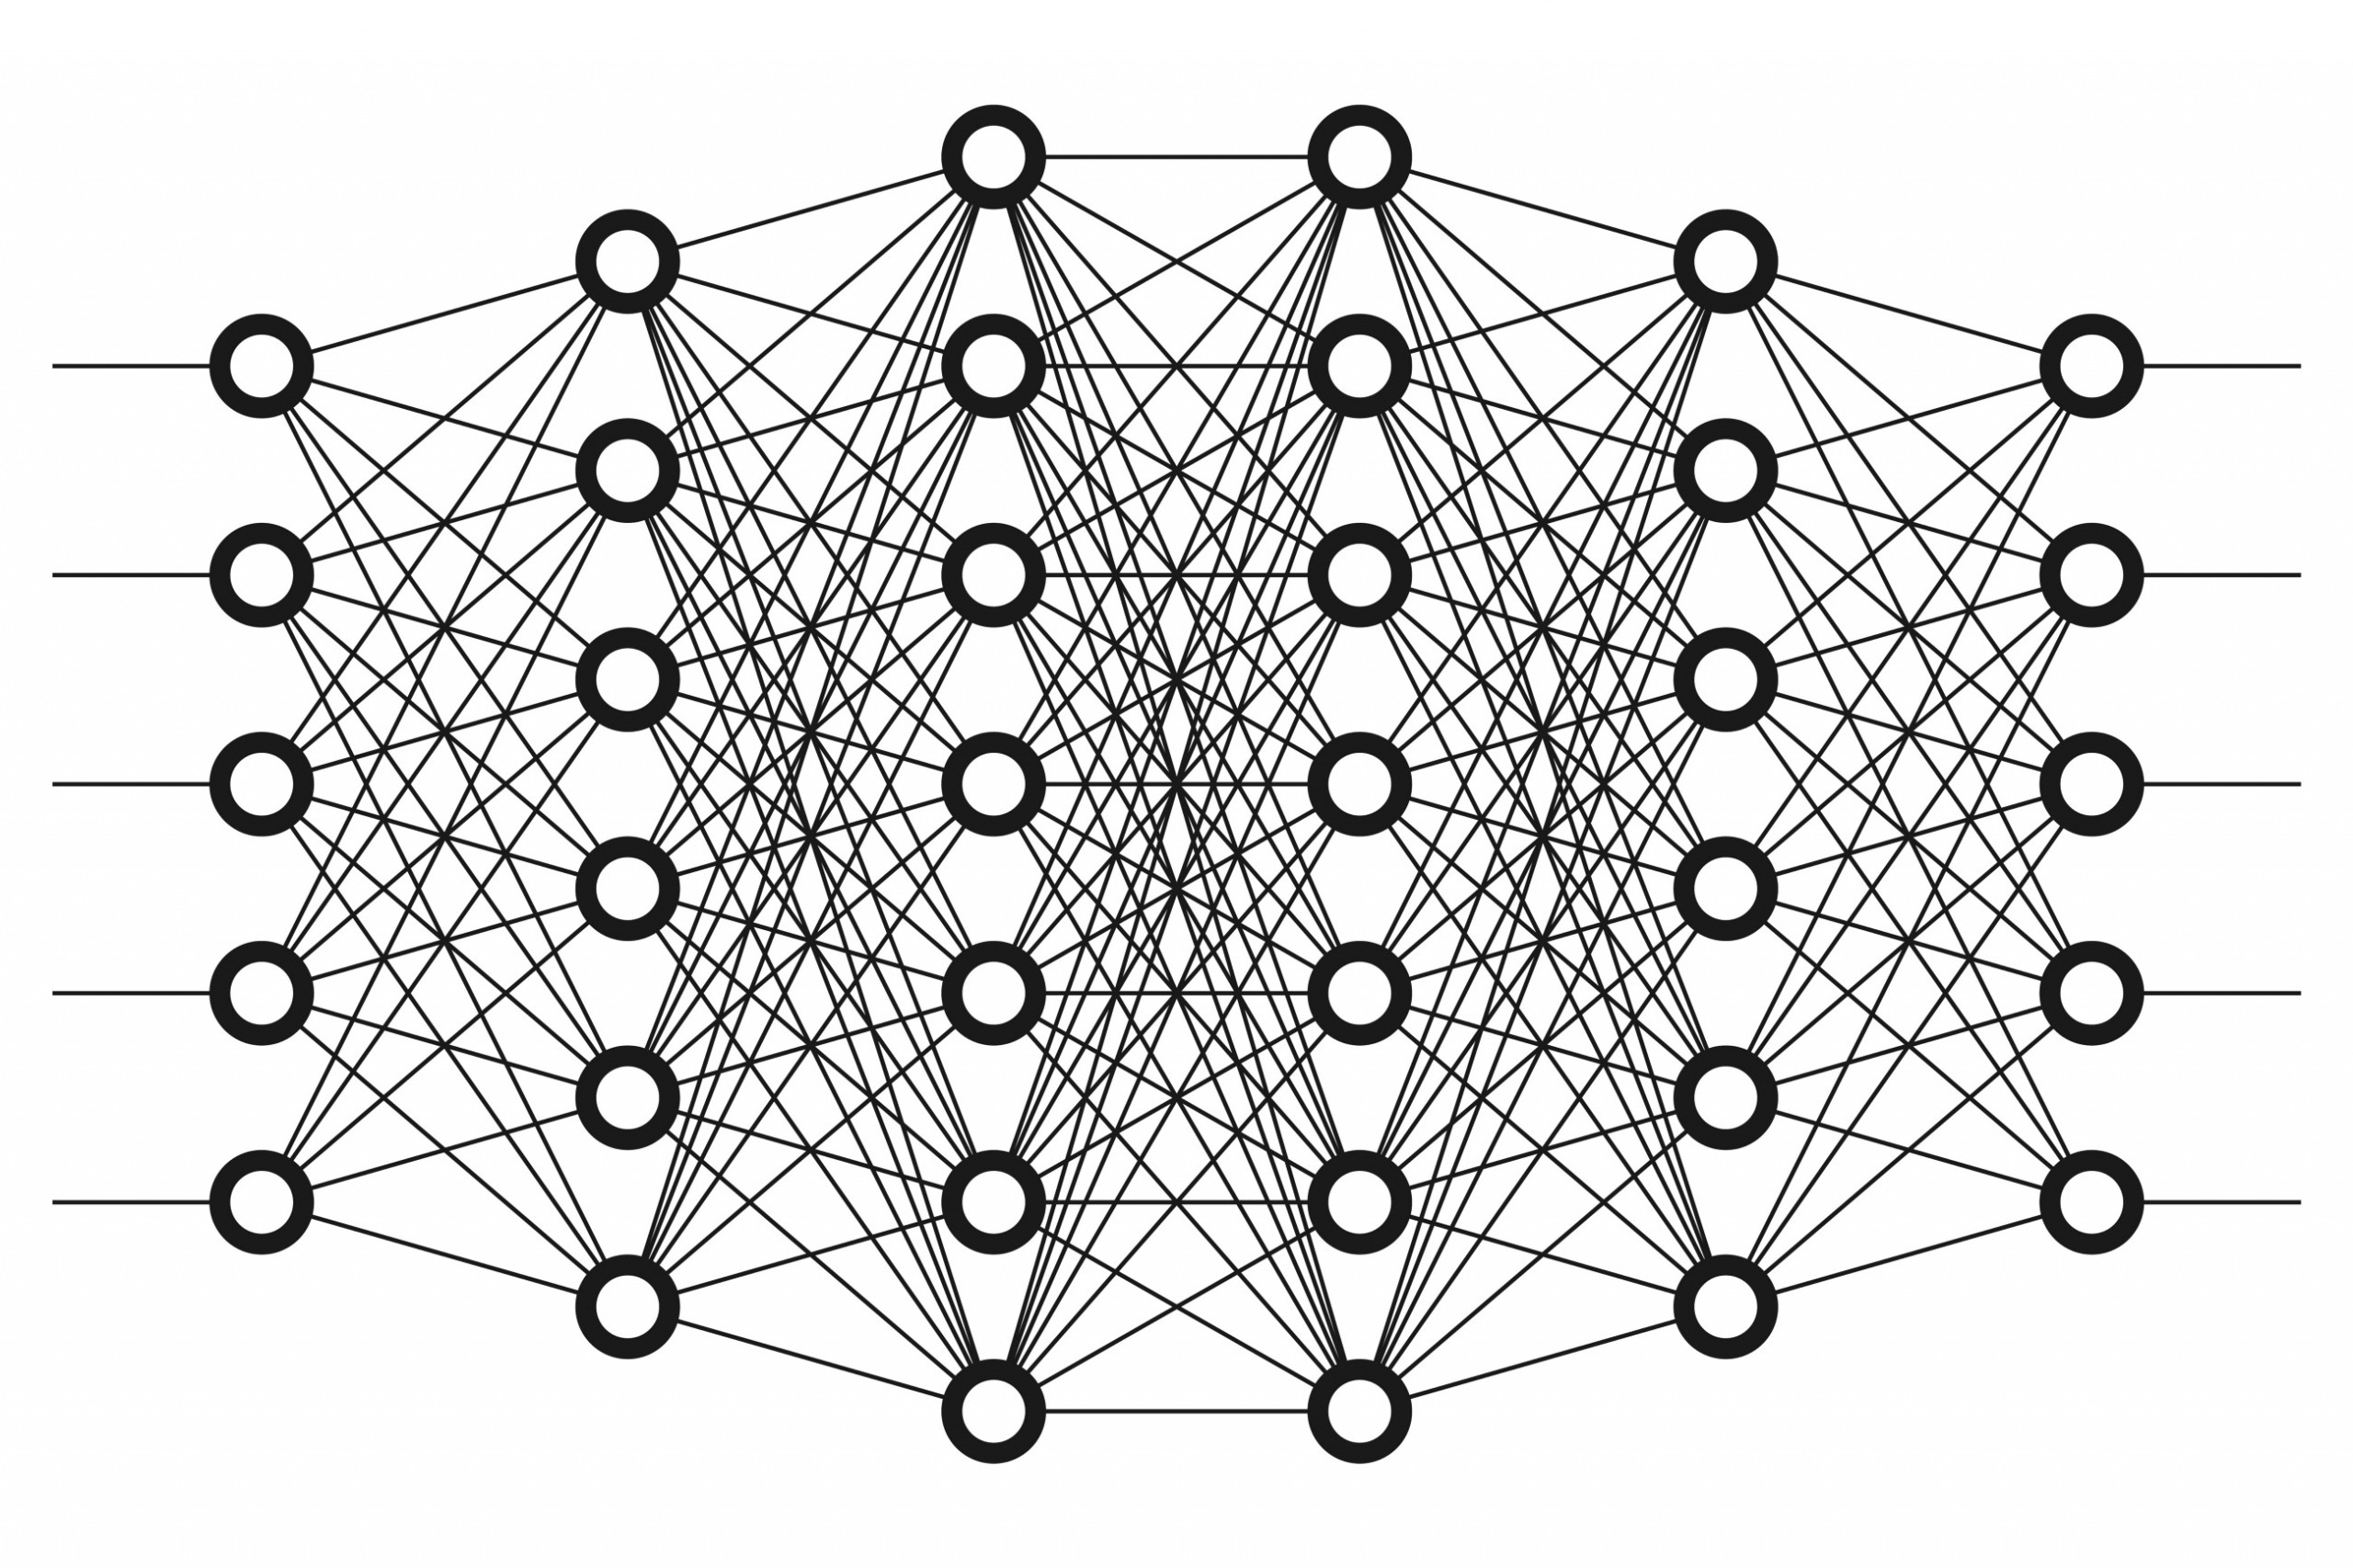
\includegraphics[width=0.8\textwidth]{figures/dnn-complex} \end{center}
\end{columns}
\end{frame}


\begin{frame}{Perceptron/Node}
\begin{center} 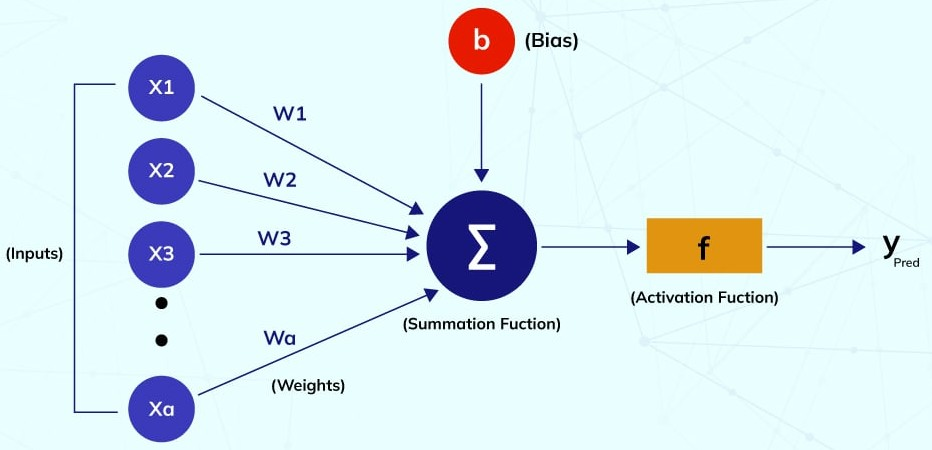
\includegraphics[width=0.8\textwidth]{figures/perceptron} \end{center}
As the goal is binary classification, an output layer with a single node is used.
\par
This node uses the \textit{Sigmoid} activation function, making the model output a fraction between 0 and 1; the probability of the input being negative or positive instance.
\end{frame}


\begin{frame}{SRNNs}
\par
\textit{Simple Recurrent Neural Networks}: a modified variation of DNNs with the ability to take multiple instances into account simultaneously.
\par
Useful for timeseries data where the changes between the values over time is as important as the values themselves.
\par
Suffers from the "vanishing gradient" problem, were the importance of older instances diminishes resulting in neglected observations.
\end{frame}


\begin{frame}{LSTMs}
\textit{Long Short Term Memory}, or LSTMs: a modified variation of SRNNs that attempts to solve the vanishing gradient issue.
\par
Adds three "gates" in each node, where each gate controls what information is going to be forgotten, remembered or passed on.
\end{frame}


\begin{frame}{GRUs}
\textit{Gated Recurrent Units}, or GRUs, use another gating mechanism to mitigate the vanishing gradient problem.
\par
Compared to LSTMs they are newer and uses a more computationally efficient gating mechanism.
\end{frame}


\section{Hyperparameter Tuning}


\begin{frame}{Hyperparameter Tuning}
Every DL model has a set of internal and external hyperparameters.
\begin{itemize}
	\item Internal hyperparameters are optimized by the model to fit the training data, such as weights and biases.
	\item External hyperparameters cannot be changed as they are part of the model itself, such as layer/node count.
\end{itemize}
You can not change the tires of a car while driving.
\end{frame}


\begin{frame}{Common Tuning Methods}
Some common methods used for finding the optimal hyperparameters:
\begin{itemize}
	\item \textbf{Random search:} Random hyperparameters are tested. After N iterations or seconds the best performing combination is used.
	\item \textbf{Grid search:} All possible hyperparameters combinations are tested. It is certain to give the optimal hyperparameters, at large computational costs.
\end{itemize}
\end{frame}


\begin{frame}{Genetic Tuning}
In this study, a genetic algorithm was used. These have shown to be highly promising for tuning.
\begin{enumerate}
	\item A population of 100 "candidates" were generated. Each candidate is a combination of external hyperparameters.
	\item A fitness value is calculated for every candidate, were the fitness is essentially its accuracy with a small penalty for training time.
	\item The top 10\% best performing candidates immediately survive to the next generation.
	\item The rest of the population is replaced by sampling two sequences of candidates, with the probability of selection proportional to their fitness.
	\item The two sequences are merged to create "offspring", inheriting its values from either parent and a 5\% chance of random mutation.
\end{enumerate}
\end{frame}


\begin{frame}{Evolution Tree}
\begin{center}
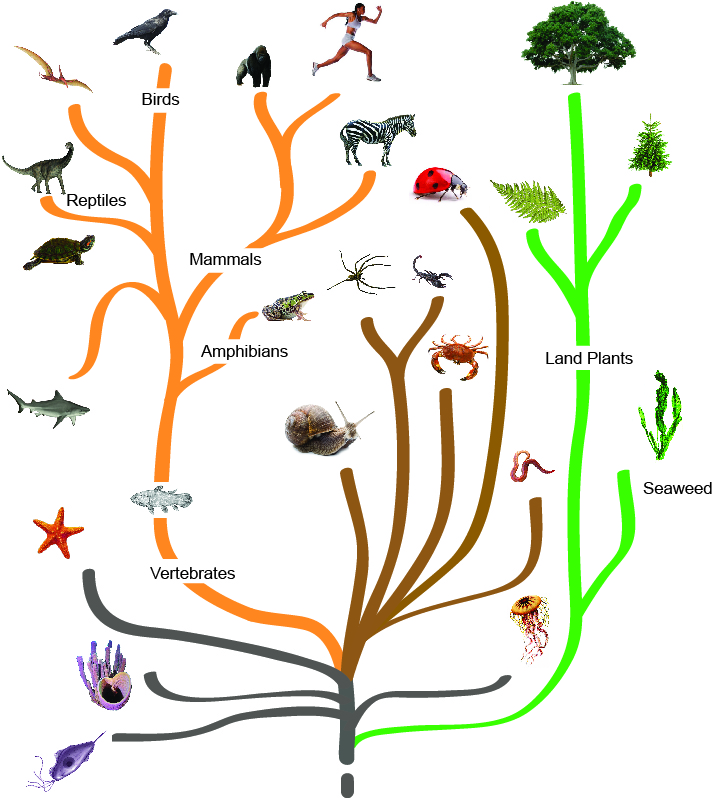
\includegraphics[width=0.6\textwidth]{figures/evolution-tree}
\end{center}
\end{frame}


\begin{frame}{Tuning Results}
Due to hardware restrictions, only three generations were able to be simulated, making it somewhat better than a random search.
\par
The following hyperparameters were produced:
\begin{itemize}
	\item Batch size: 128
	\item Optimizer: adam
	\item Activation function for the recurrent layers: tanh
	\item Activation function for the dense layers: relu
	\item Dropout for the recurrent layers: 0.2
	\item Dropout for the dense layers: 0.2
	\item Number of recurrent layers: 2
	\item Number of dense layers: 0
	\item Number of units in the recurrent layers: 256
	\item Number of units in the dense layers: 64
	\item Normalization between recurrent layers: yes
	\item Normalization between dense layers: yes
\end{itemize}
\end{frame}


\section{Model Evaluation}


\begin{frame}{Timeframes \& lookback/lookahead}
In order to assess models over timeframes, two evaluation factors \textit{lookback} and \textit{lookahead} are introduced.
\begin{description}
	\item[Lookback] is the number of time steps to take into account when making a prediction.
	\item[Lookahead] is the of number of time steps within which to make a prediction.
\end{description}
\end{frame}


\begin{frame}[fragile]{Timeframe restructuring}
Modifying the data based on lookback is simple, just use the $n$ last observations.
\par
Modifying based on lookahead is more complicated. Simply increasing the lookahead period still means the lightning strike always occur within the first hour.
\begin{semiverbatim}
	_ _ x x x x | y
	_ x x x x | _ y
	x x x x | _ _ y
\end{semiverbatim}
\end{frame}


\begin{frame}[fragile]{Timeframe restructuring}
Furthermore, within the newly created lookahead sequence, another independent lightning strike might have occurred.
\begin{semiverbatim}
	x x x x | _
	x x x x | _ _ z
\end{semiverbatim}
\par
This will increase the number of positive classes, and at this point it is not feasable to repopulate negative instances.
\par
To accomodate for this, class weights are used as a last resort.
\end{frame}


\begin{frame}{Stratified k-fold cross validation}
A strategy for testing, with the purpose of minimizing randomness and luck. In this study $k=10$.
\begin{enumerate}
	\item Split the data into 10 different partitions, where each partition contains an equal number of positive and negative instances.
	\item Iterate through the training and evaluation phase k times, with each iteration using a different partition as test set and the remaining partitions as training set.
	\item Calculate the evaluation metric for each iteration. Set the final evaluation metric as the mean.
\end{enumerate}
\end{frame}


\begin{frame}{Metrics}
The following metrics were collected for each model:
\begin{itemize}
	\item \textbf{Training Time:} The time it takes to train the model. Provides an indication of its computational requirements.
	\item \textbf{Accuracy:} A simple and widely used metric providing the frequency of correct predictions made by a model.
	\item \textbf{F1-Score:} F1-score is similar to accuracy, but also takes class balance into account.
	\item \textbf{Mean Absolute Error:} A metric that provides insight into the general confidence of the models.
\end{itemize}
\end{frame}


\section{Model Performance}


\begin{frame}{Model Performance: DNN}
\begin{itemize}
	\item Very short training time of ~9s.
	\item Good accuracy overall of 88-89\%.
	\item Very concistent performance across lookahead values (mean diffence of 0.15\%).
	\item Remember, lookback is constant for this model.
\end{itemize}
\end{frame}


\begin{frame}{Model Performance: SRNN}
\begin{itemize}
	\item Highest training time of ~130s.
	\item Highest overall accuracy, avaraging 89-90\%.
	\item Most confident model overall.
\end{itemize}
\end{frame}


\begin{frame}{Model Performance: LSTM}
\begin{itemize}
	\item Decent training time of ~58s.
	\item Highest accuracy for shorter lookback/lookahead combinations (~92\%).
	\item Sharp dropoff in accuracy once $\text{lookback} > 1, \text{lookahead} > 6$.
\end{itemize}
\end{frame}


\begin{frame}{Model Performance: GRU}
\begin{itemize}
	\item Very similar to the LSTM model, but slightly better across all metrics.
	\item ~9s shorter training time.
	\item Fractional accuracy increase.
\end{itemize}
\end{frame}


\section{Findings and Observations}


\begin{frame}{Model Comparison}
Which model is the best? Depends on the use-case.
\begin{itemize}
	\item If only short lookback/lookahead combinations are required, the GRU model can yield up to 4\% better accuracy than DNN/SRNN models.
	\item If higher lookahead is required, DNN or SRNN models are recommended.
	\begin{itemize}
		\item DNNs significantly faster, at the cost of slightly lower accuracy.
	\end{itemize}
	\item If high lookback and lookahead is required, the SRNN model is recommended.
\end{itemize}
\end{frame}


\begin{frame}{Findings}
LSTM and GRU models, specifically designed for timeseries prediction, performs better when not concidering the timeseries aspect.
\par
Using timeseries only seems to confuse the models.
\end{frame}


\begin{frame}{Challanges and limitations}
\begin{itemize}
	\item \textbf{Generalization:} Getting the model to transfer its knowledge across different geographic locations and topologies.
	\item \textbf{Data Availability:} Data may vary based on location, source and standardization.
	\item \textbf{Interpretability:} DL models are notoriously difficult to understand. Similar to a surgeon trying to understand the thoughtprocess of a patient by looking at their brain.
\end{itemize}
\end{frame}


\begin{frame}{Improvements and future work}
\begin{itemize}
	\item \textbf{Dataset:} Increasing the dataset. In this study only 50,000 of 3,000,000 lightning strikes could be used. Experimenting with different parameters might also be beneficial.
	\item \textbf{Different topologies:} Examining model performance across different topologies and environments. Is it possible to include topological data as input parameters?
	\item \textbf{Model architecture:} Exploring more complex architectures such as convolution/recurrent hybrids. Running the genetic tuning process for longer periods of time is also recommended.
	\item \textbf{Better dataset balance:} Currently, there is likely significant differences between positive and negative instances. A better evaluation would take more similar and realistic instances into account.
\end{itemize}
\end{frame}


\section{Fin}


\begin{frame}{Fin}
\centering
Fin
\end{frame}


\end{document}
